\chapter{逻辑结算}\label{sec7}

\begin{introduction}
\item MechScope模组
\item 逻辑帧
\item 爆门
\item 逻辑同步
\item 逻辑延迟
\end{introduction}

在上一章中我们介绍了很多电路模块。这时候读者如果想当然地把这些电路模块组合起来,容易发生一些意想不到的问题,这也是上一章没有介绍过多复合电路的原因。在这一章中,我们将完善整个逻辑结算中的所有细节,确保可以预测任何复合逻辑电路的行为。

在一个逻辑电路中,每个电源和用电器可以接多根线,每根线可以接多个电源和用电器。当电路激活时,所有电源、电线、用电器都会按照一定顺序激活。

非常明显的结论是,电源激活后,电源上的电线激活,然后电线下的用电器激活。进一步的,如果电源$A$比电源$B$先激活,那么电源$A$上的电线也应当比$B$上的电线先激活;如果电线$a$比电线$b$先激活,那么$a$下的所有用电器也应当比$b$下的所有用电器先激活;如果逻辑门$A$上的逻辑灯比逻辑门$B$上的逻辑灯先激活,那么逻辑门$A$也应当比逻辑门$B$先激活。

以上的一些规则都是合理的,很容易理解。接下来的规则则是泰拉瑞亚特有的,需要进行记忆。

当一个电源激活后,其上的四色电线,按照红、蓝、绿、黄的先后顺序激活。

当一根电线激活后,其上各点按照距离电源由近到远的顺序激活。到电源距离相等的点,理解激活顺序需要理解图的广度优先搜索(BFS)算法,这里不详细解释。

对于涉及到逻辑门的电路,电路结算被分步进行。每一步中都进行逻辑门激活——电线激活——逻辑灯激活——逻辑门判断这四小步。逻辑灯被激活后,暂时不进行逻辑判断,等到所有电线结算完毕后,再统一进行逻辑判断。这每一步叫做\textbf{逻辑帧}。一个逻辑电路的结算过程中,反复运行每个逻辑帧中的四小步,直到没有逻辑门需要激活。

除了逻辑门以外的电源叫做\textbf{物理电源}。一个逻辑结算必须通过物理电源的激活启动。一个逻辑结算中一个逻辑门只能激活至多一次。如果它尝试激活第二次,那么激活失败并有白烟从逻辑门发出,称为\textbf{爆门}。逻辑门状态仍然会正常切换但是不会发出信号。爆门属于正常机制,是开发者有意为之,加以利用也可以起到作用。

\section{用 MechScope 模组研究电路结算过程}
MechScope 模组可以将电路结算过程可视化。其下载链接已经在\autoref{sec1:1}中给出。安装该模组后,在游戏内可以看到电路的结算过程。

\begin{figure}[!ht]

\includegraphics[width=0.95\textwidth]{images/273.png}
\caption{MechScope模组}\label{i273}
\end{figure}

进入游戏后,打开设置——控制,可以看到MechScope的键位设置。默认键位为:
\begin{itemize}
\item[小键盘1] Toggle(触发)
\item[小键盘2] Step(步进)
\item[小键盘3] Auto Step(自动步进)
\item[小键盘5] Settings(设置)
\end{itemize}

如\autoref{i274}所示,先做一个最简单的电路。在这个电路中,开关通过一根红线控制火把。
\begin{figure}[!ht]
\begin{center}
\subfloat[]{\label{i274}
\includegraphics{images/274.png}}
\qquad
\subfloat[]{\label{i277}
\includegraphics{images/277.png}}
\end{center}
\caption{}
\end{figure}

按下小键盘1,可以看到光标右上角有一个黄点(\autoref{i275}),表示MechScope正在运行。
\begin{figure}[!ht]
\begin{center}
\subfloat[]{\label{i275}
\includegraphics{images/275.png}}
\qquad
\subfloat[]{\label{i276}
\includegraphics{images/276.png}}
\end{center}
\caption{}
\end{figure}

右键点击开关,此时电路会被暂停。开关上显示一个红框,电线所在格加了一层红色滤镜,分别表示激活的电源和电线(\autoref{i277})。火把已经熄灭。光标右上角的黄点变成了红点(\autoref{i276}),表示有正在运行的电路。按一下小键盘2进行步进,电路结算完成,光标右上角恢复黄点。

了解了基本操作,我们来看设置菜单。按下小键盘5,打开设置菜单(\autoref{i278})。前四项是单选,表示每次步进的幅度。Single是逐格步进,Wire是逐线步进,Source是逐源步进,Stage是逐逻辑帧步进。后六项是显示设置,仅影响可视化程度,这里不进行介绍,读者可自行尝试。最后一个数字是自动步进的周期/物理帧,这个值越小,自动步进越快。
\begin{figure}
\centering
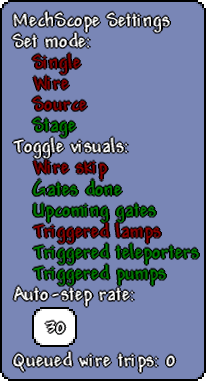
\includegraphics[width=0.3\textwidth]{images/278.png}
\caption{MechScope的设置菜单}\label{i278}
\end{figure}

我们的重心放在前四项设置,它们是有关于电路结算的,其中Stage是关于逻辑结算的。

\subsection{逐格步进}
设置菜单中选择逐格步进,然后做出\autoref{i274_2}所示的电路。打开MechScope,右键点击开关,可以看到开关上出现了红框,表示开关作为电源,激活了它上面的红线(\autoref{i279})。按下小键盘2步进,开关右边一格出现了红框,表示这一格激活(\autoref{i280})。反复步进,红框一直向右移动直到火把上,把火把关闭。
\begin{figure}
\begin{center}
\subfloat[]{\label{i274_2}
\includegraphics[width=0.27\textwidth]{images/274.png}}\\
\subfloat[]{\label{i279}
\includegraphics[width=0.27\textwidth]{images/279.png}}
\qquad
\subfloat[]{\label{i280}
\includegraphics[width=0.27\textwidth]{images/280.png}}
\qquad
\subfloat[]{\label{i281}
\includegraphics[width=0.27\textwidth]{images/281.png}}
\qquad
\subfloat[]{\label{i282}
\includegraphics[width=0.27\textwidth]{images/282.png}}
\qquad
\subfloat[]{\label{i283}
\includegraphics[width=0.27\textwidth]{images/283.png}}
\qquad
\subfloat[]{\label{i284}
\includegraphics[width=0.27\textwidth]{images/284.png}}
\end{center}
\caption{}
\end{figure}

这个实验展示了单根电线上的激活顺序:电线由近到远依次激活。不过它只展示了单向传播的情况。对于复杂的情况,读者可以自己使用MechScope模组研究。一般情况下我们只需要知道距离电源近的先激活,距离电源远的后激活,这里的距离指沿电线到电源最短路径的长度。这里为计算机专业的同学提供一个信息:单根电线是按照从电源开始广度优先搜索的顺序激活的,四个方向的顺序是下上右左。

\subsection{逐线步进}
设置菜单中选择逐线步进,然后做出\autoref{i285}所示的电路。在逐线步进模式下,每次步进会前进一整根电线。右键点击开关,可以看到红线激活(\autoref{i286});步进,蓝线激活(\autoref{i287});步进,绿线激活(\autoref{i288});步进,黄线激活(\autoref{i289})。
\begin{figure}
\begin{center}
\subfloat[]{\label{i285}
\includegraphics[width=0.27\textwidth]{images/285.png}}
\qquad
\subfloat[]{\label{i286}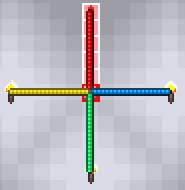
\includegraphics[width=0.27\textwidth]{images/286.png}}
\qquad
\subfloat[]{\label{i287}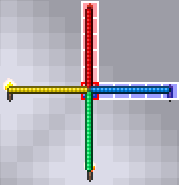
\includegraphics[width=0.27\textwidth]{images/287.png}}
\qquad
\subfloat[]{\label{i288}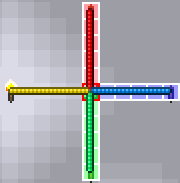
\includegraphics[width=0.27\textwidth]{images/288.png}}
\qquad
\subfloat[]{\label{i289}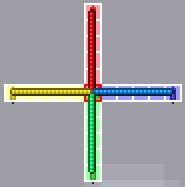
\includegraphics[width=0.27\textwidth]{images/289.png}}
\end{center}
\caption{}
\end{figure}

这个实验展示了单个电源上不同电线的激活顺序:红线、蓝线、绿线、黄线依次激活。

\subsection{逐逻辑帧步进}
我们先跳过逐源步进,来看逐逻辑帧步进。电路如\autoref{i290}所示。在逐逻辑帧步进模式下,每次步进会前进一个逻辑帧。
\begin{figure}
\begin{center}
\subfloat[]{\label{i290}
\includegraphics[width=0.27\textwidth]{images/290.png}}\\
\subfloat[]{\label{i291}
\includegraphics[width=0.27\textwidth]{images/291.png}}
\qquad
\subfloat[]{\label{i292}
\includegraphics[width=0.27\textwidth]{images/292.png}}
\qquad
\subfloat[]{\label{i293}
\includegraphics[width=0.27\textwidth]{images/293.png}}
\qquad
\subfloat[]{\label{i294}
\includegraphics[width=0.27\textwidth]{images/294.png}}
\qquad
\subfloat[]{\label{i295}
\includegraphics[width=0.27\textwidth]{images/295.png}}
\qquad
\subfloat[]{\label{i296}
\includegraphics[width=0.27\textwidth]{images/296.png}}
\end{center}
\caption{}\label{i290:296}
\end{figure}

我们一般把物理电源激活时的逻辑帧记作第0个逻辑帧(\autoref{i291}),往后每个逻辑帧都进行逻辑门激活,电线激活,逻辑灯激活,逻辑门判断。在\autoref{i290:296}中,从\subref{i291}到\subref{i296}分别是第0个逻辑帧到第5个逻辑帧,每个逻辑帧中都用加粗方框标出了激活的逻辑门,滤镜标出了激活的电线,“×”标出了已经激活过的逻辑门,“○”标出了在下一逻辑帧将要激活的逻辑门。

\begin{figure}
\begin{center}
\subfloat[]{\label{i297}
\includegraphics[width=0.45\textwidth]{images/297.png}}\\
\subfloat[]{\label{i298}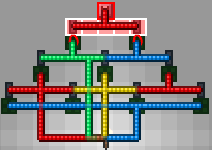
\includegraphics[width=0.45\textwidth]{images/298.png}}
\qquad
\subfloat[]{\label{i299}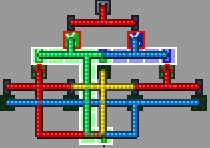
\includegraphics[width=0.45\textwidth]{images/299.png}}
\qquad
\subfloat[]{\label{i300}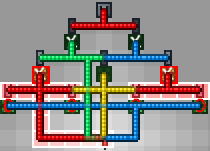
\includegraphics[width=0.45\textwidth]{images/300.png}}
\qquad
\subfloat[]{\label{i301}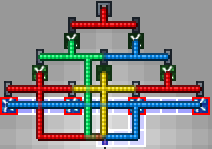
\includegraphics[width=0.45\textwidth]{images/301.png}}
\end{center}
\caption{}\label{i297:301}
\end{figure}

再来看一个稍复杂的电路(\autoref{i297})。右键点击开关,进入第0个逻辑帧(\autoref{i298}):开关作为电源激活,开关上的红线激活,两个逻辑灯激活,两个逻辑门进行判断,并计划激活(逻辑门上画了一个小的红圈)。

第1个逻辑帧(\autoref{i299})。两个逻辑门作为电源激活,蓝线和绿线激活,三个逻辑灯及火把激活。其中火把改变状态,左右两个逻辑灯改变状态,中间的逻辑灯因为激活了两次,状态不变。三个逻辑灯下的逻辑门进行判断,其中左右两个逻辑门计划激活,中间的逻辑门不计划激活。

第2个逻辑帧(\autoref{i300})。两个逻辑门作为电源激活,两根红线激活,四个逻辑灯及火把激活,全部改变状态。四个逻辑门计划激活。

第4个逻辑帧(\autoref{i301})。四个逻辑门作为电源激活,蓝线激活四次,火把激活四次,状态不变。没有计划激活的逻辑门,逻辑结算结束。

\subsection{爆门}

来看\autoref{i302},这是一个循环电路,看起来,红线在第0个逻辑帧激活,蓝线在第1个逻辑帧激活,红线又在第2个逻辑帧激活,蓝线又在第三个逻辑帧激活……如果真是这样,那么游戏会崩溃,因为泰拉瑞亚中,无论电路有多复杂,都必须要在一个物理帧内结算完毕。如果1/60秒没法结算完的话,物理帧会相应的加长,导致帧率降低。如果永远结算不完,那么游戏就会卡在一个物理帧中,无法进行任何操作。

泰拉瑞亚使用了一种傻瓜方法来规避这种死循环。一个逻辑门激活后,会有一个标记,在MechScope中会显示一个白色的“×”。如果之后这个逻辑门还计划激活(MechScope显示红色的“○”),那么取消这个计划,并且播放爆门动画(冒烟)。在\autoref{i302:305}中,爆门的行为发生在\autoref{i305},即上面的逻辑门再次计划激活时。截图没能截下爆门的瞬间,读者可以自行尝试。

\begin{figure}
\begin{center}
\subfloat[]{\label{i302}
\includegraphics[width=0.1\textwidth]{images/302.png}}
\qquad
\subfloat[]{\label{i303}
\includegraphics[width=0.1\textwidth]{images/303.png}}
\qquad
\subfloat[]{\label{i304}
\includegraphics[width=0.1\textwidth]{images/304.png}}
\qquad
\subfloat[]{\label{i305}
\includegraphics[width=0.1\textwidth]{images/305.png}}
\end{center}
\caption{}\label{i302:305}
\end{figure}

之所以称之为“傻瓜方法”,是因为它有副产物。换句话讲,对于不会死循环的电路也会发生爆门。在\autoref{i306:308}中,下方的逻辑门在第1个逻辑帧激活,并被标记了“×”。第1个逻辑帧中,蓝线激活,下方的逻辑灯状态改变,所以逻辑门又要计划激活,结果爆门。

\begin{figure}
\begin{center}
\subfloat[]{\label{i306}
\includegraphics[width=0.1\textwidth]{images/306.png}}
\qquad
\subfloat[]{\label{i307}
\includegraphics[width=0.1\textwidth]{images/307.png}}
\qquad
\subfloat[]{\label{i308}
\includegraphics[width=0.1\textwidth]{images/308.png}}
\end{center}
\caption{}\label{i306:308}
\end{figure}

从上面两个例子中我们总结一下爆门的原因。一个逻辑门在一次电路结算中至多只会激活一次。如果尝试再次激活,那么激活失败并爆门。需要注意的是,逻辑门状态仍会照常改变。

在实际应用中,爆门经常导致电路bug,这是因为我们往往希望逻辑门在多次状态切换时可以多次激活,但实际上不会。学会了预测爆门,就可以想办法避免爆门,甚至利用爆门。

\section{逻辑延迟器}

在连接多个逻辑电路模块时,要让它们正确地合作,就需要控制它们的运行顺序。不同电路模块从输入到输出经历的逻辑帧数量不同,所以简单的接线方式可能使得一些模块在不该工作时工作,打乱电路状态。使用逻辑延迟器可以推迟一个电路模块的运行逻辑帧,使得这个电路模块在需要运行的时候才运行。

上一章讲到的换线器就可以作为逻辑延迟器,因为输出激活比输入激活晚一个逻辑帧。如果将多个换线器首尾连接,就可以控制延迟的逻辑帧数量。逻辑延迟器的常见套路见\autoref{i153:156}。

\begin{figure}[!ht]
\begin{center}
\subfloat[横式]{

\includegraphics{images/153.png}
}
\qquad
\subfloat[竖式]{
\quad
\includegraphics{images/154.png}\quad
}
\qquad
\subfloat[斜式]{

\includegraphics{images/155.png}
}
\qquad
\subfloat[双竖式]{
\quad
\includegraphics{images/156.png}\quad
}
\subfloat[紧凑横式,利用了爆门]{

\includegraphics{images/157.png}
}
\end{center}
\caption{逻辑延迟器的不同摆法,逻辑延迟均为3个逻辑帧。}
\label{i153:156}
\end{figure}

\section{网线}\label{sec17}
在设计大型电路时,有时会遇到需要在两地之间传递复杂信号的情况,例如在A地设置多个传感器,在B地进行处理并响应。一般来说每个信号都需要接一根线,这样一来当信号较复杂时,接线会占用非常大的空间。这是由于一根电线能传递的信号复杂度太低:一根电线只能选择激活或不激活两种状态,所以每根电线只能传递一个二进制位。

在了解了逻辑结算机制以后,我们可以使用一根电线传递多个二进制位。这个功能与现实生活中网线的功能类似,所以我们把它称为网线。因为逻辑门是对逻辑帧敏感的,我们可以将多个二进制位在不同的逻辑帧通过一根电线发送出,并在接收端将这些信息解析。归根到底,我们需要做一个编码器和一个解码器。编码器用来把多根线上的简单信号翻译为一根线上的复杂信号,解码器用来将一根线上复杂信号翻译为多根线上的简单信号。

编码器和解码器的设计取决于信号特点,因此这里不给出固定的做法,仅给出一个简单例子作参考。我们在A地放置8根火把,使用开关可以改变它们的状态;在B地放置8根火把;A地和B地之间只能通过1根线连接。我们希望在设置完A地的火把之后,触发一个开关,就可以把A地的火把状态更新到B地,即利用一根线传递八个二进制位。在发送端电路中,读者需要学习到如何利用逻辑延迟器在某个特定的逻辑帧发送信号;在接收端电路中,读者需要学习如何利用故障逻辑门判断一根线是否在某个特定的逻辑帧激活。

\begin{figure}[!ht]
\centering

\includegraphics{images/239.png}\qquad
\includegraphics{images/240.png}
\caption{8个开关分别控制8个火把的状态,控制杆用来发送信号,黄线用来输出。第0个逻辑帧黄线激活,用来做启动信号,随后通过上方的逻辑延迟器,8个D锁存器依次在1\~{}8个逻辑帧激活。}
\label{i239:240}
\end{figure}

在A地,我们需要在8个逻辑帧中依次触发对应的D触发器,把信号发送出去(\autoref{i239:240})。

\begin{figure}[!ht]
\centering

\includegraphics{images/241.png}\qquad
\includegraphics{images/242.png}
\caption{接收到黄线(在第0个逻辑帧)的激活时开始工作。上方的逻辑延迟器依次在1\~{}8个逻辑帧将下方对应的有效逻辑灯点亮,对应逻辑帧时如果黄线激活,那么下方对应的火把被激活。第9个逻辑帧复位。}
\label{i241:242}
\end{figure}

在B地,我们需要把各个逻辑帧的输入提取出来,然后分别输出给8个火把(\autoref{i241:242})。

以上的装置虽然使用了很多逻辑门,但是当AB两地距离较远时,使用这些逻辑门总比使用8根电线连接AB两地要好。

\section{普通逻辑门的逻辑同步}
对于有数电基础的玩家,刚涉及泰拉瑞亚电路时会遇到各种各样的爆门。而通过各种各样教学视频入门的“外行”反而不容易遇到这样的问题。

爆门的原因是一个逻辑门在一次逻辑结算中激活多次。虽然故障逻辑门也可以发生爆门(下一小节会讲),但是普通逻辑门才是爆门的重灾区。我们在使用普通逻辑门的时候,一般都是要进行简单的组合逻辑运算,比如几个与逻辑,几个异或逻辑的结合。这样的逻辑运算当然是可以进行状态判断的而不需要使用激活判断。可以进行状态判断的前提是,一根线连接的所有电源和用电器的状态要同步,换句话就是,电源状态改变时,和电源连接的所有用电器状态也要改变。但是当爆门发生时,逻辑门状态改变却不发出信号,这样就会导致用电器状态不变,电路就无法进行状态判断了。不能进行状态判断的电路就没办法做组合逻辑。

举一个简单的例子。我们知道降频电路(\autoref{sec2:1})可以做二进制计数,而\autoref{sec2:2}中的电路可以将二进制编码转成十进制显示。那么自然而然就会想到,把这两个电路连起来不就可以进行十进制计数了吗?

\begin{figure}[!ht]
\centering
\subfloat[]{\label{fig13}
\includegraphics{images/367.png}\quad
\includegraphics{images/368.png}}
\qquad
\subfloat[]{\label{fig14}
\includegraphics{images/369.png}\quad
\includegraphics{images/370.png}}
\qquad
\subfloat[]{\label{fig15}\includegraphics{images/371.png}\quad\includegraphics{images/372.png}}
\qquad
\subfloat[]{\label{fig16}\includegraphics{images/373.png}\quad\includegraphics{images/374.png}}
\qquad
\subfloat[]{\label{fig17}\includegraphics{images/375.png}\quad\includegraphics{images/376.png}}
\qquad
\subfloat[]{\label{fig18}\includegraphics{images/377.png}\quad\includegraphics{images/378.png}}
\end{figure}

这里仅给出精简版的电路来说明这样做不对。如\autoref{fig13},仅用一个降频电路,那么可以计四个数,用四个双灯与门进行解码,输出到四个火把。

开关第一次激活,仅红线激活,激活后各逻辑灯与逻辑门的状态如\autoref{fig14},所以第一个门和第二个门激活,第一个火把熄灭,第二个火把点亮。开关第二次激活,红线与蓝线都激活,但是红线比蓝线早一个逻辑帧。红线激活后各逻辑灯与逻辑门状态如\autoref{fig15},此时第一个门和第二个门激活,第一个火把点亮,第二个火把熄灭。蓝线激活后各逻辑灯与逻辑门状态如\autoref{fig16},此时第一个门和第三个门激活,但是第一个门已经激活过了,所以爆门,只有第三个门激活,所以第三个火把点亮(\autoref{fig17})。到这里可以看出来,尽管逻辑门的状态是对的,即只有第三个逻辑门是亮的,但是火把状态不对,这是因为第一个门爆门后第一个火把少了一次激活。

导致这个爆门的原因是红线比蓝线早一个逻辑帧,解决起来也很简单,那就是在红线上做一个逻辑延迟,让红线和蓝线在同一个逻辑帧激活(\autoref{fig18})。

\section{状态表示与激活表示}

泰拉瑞亚电路中的信号有两种表示方式:状态表示和激活表示。状态表示一般是显式的,即肉眼可以直接通过电路元件的状态读出其要表示的信息,例如亮表示1,灭表示0。激活表示是隐式的,激活表示1,不激活表示0。因为激活对于任何有显示效果的物品(像素盒除外)都只能改变其状态,因此想读出激活的信息,就需要在电路元件激活前和激活后的状态之间比较,状态变化的是1,状态不变的是0。这种读法显然是不方便的。

从电路运行角度,状态表示与激活表示经常需要搭配使用。普通逻辑门一般适用于状态表示,而故障逻辑门适用于激活表示。无论是为了产生可读性输出,还是为了在各电路模块之间传输信息,都会用到在状态表示与激活表示之间互换的方法。这一节中就将介绍将状态表示与激活表示互换的方法。

\subsection{状态表示转为激活表示}

一个故障逻辑门就可以做到将亮转变为激活,灭转变为不激活的功能。需要注意的是,仅用一个故障逻辑门的话,即使有效逻辑灯在一个逻辑结算中多次在亮灭之间切换,逻辑门也至多只能激活一次。所以更细分,有点亮立刻激活(\autoref{i173:175}\subref{i174})与事后激活(\autoref{i173:175}\subref{i175})两种造法。

\begin{figure}[!ht]
\begin{center}
\subfloat[]{
\label{i173}
\includegraphics{images/173.png}
}
\qquad
\subfloat[]{
\label{i174}
\includegraphics{images/174.png}
}
\qquad
\subfloat[]{
\label{i175}
\includegraphics{images/175.png}
}
\end{center}
\caption{红线控制有效逻辑灯状态。\protect\subref{i174}有效逻辑灯点亮时立刻激活;\protect\subref{i175}事后激活,在某个时刻激活蓝线可以将有效逻辑灯的亮/灭转换为故障逻辑门的激活/不激活。}
\label{i173:175}
\end{figure}

点亮瞬间激活使用的就是降频电路,这里不作详细解释。事后激活即在某个时候(逻辑帧)中对于状态为1的激活,状态为0的不激活。

\subsection{激活表示转为状态表示}

激活转状态,需要将激活转变为点亮,不激活转变为熄灭。电路设计时需要特别注意“不激活”时的响应,因为按照电路原理,不激活时是不会有用电器响应的。如果要响应“不激活”,就必须在某个时间令电路执行不激活时的响应,见\autoref{i173:176}。

\begin{figure}[!ht]
\begin{center}
\subfloat[]{
\label{i173b}
\includegraphics{images/173.png}
}
\qquad
\subfloat[]{
\label{i176}
\includegraphics{images/176.png}
}
\end{center}
\caption{无论红线是否激活,首先激活蓝线将有效逻辑灯置0,随后红线激活则有效逻辑灯变为1,否则有效逻辑灯为0。}
\label{i173:176}
\end{figure}

\subsection{可以随机显示的十进制数显}

上一章我们做的十进制数显输入还不够自由:要么需要输入二进制,要么需要连续数字。一个完美意义下的十进制数显应该接收11个输入,前十个输入激活则显示0\~{}9的数字,最后一个输入激活则全部熄灭。

显示0\~{}9的数字对应的是火把状态,而输入是激活。因此需要一个将激活转化为状态的电路。如\autoref{i127:128},在火把上加上事前置0电路。无论激活哪个开关,事前置0电路都会在第0个逻辑帧激活,在第1个逻辑帧生效。显示电路在第0个逻辑帧激活,在第1至2个逻辑帧生效。

\begin{figure}[!ht]
\begin{center}
\subfloat{
\label{i127}
\includegraphics[width=0.45\textwidth]{images/127.png}
}
\qquad
\subfloat{
\label{i128}
\includegraphics[width=0.45\textwidth]{images/128.png}
}
\end{center}
\caption{}
\label{i127:128}
\end{figure}

\section{双激活技术}\label{sec33}
双激活技术,指在两个相邻逻辑帧激活同一个逻辑灯的做法。双激活一般通过\autoref{fig43}实现。双激活有很多种用途。
\begin{figure}[!ht]
\centering
\includegraphics{images/421.png}
\caption{第一次激活红线时,由于逻辑门的影响,在紧接着的逻辑帧中红线还会再激活一次。由于爆门机制,红线不会激活第三次。}\label{fig43}
\end{figure}

\subsection{普通逻辑门的状态转激活}
普通逻辑门的状态转激活有三种常见做法,见\autoref{fig44}。

\begin{figure}[!ht]
\centering
\subfloat[与门从灭变亮时激活,从亮变灭不激活。]{\label{fig45}\quad\qquad\includegraphics{images/422.png}\quad\includegraphics{images/423.png}\qquad\qquad}
\qquad
\subfloat[与门亮时故障逻辑门可以激活,灭时不可以激活。]{\label{fig46}\qquad\qquad\includegraphics{images/424.png}\qquad\qquad}
\qquad
\subfloat[与门亮时故障逻辑门可以激活,灭时不可以激活。]{\label{fig47}\quad\qquad\qquad\includegraphics{images/425.png}\qquad\qquad\quad}
\caption{}\label{fig44}
\end{figure}

\autoref{fig45}使用了降频电路实现两次激活变一次激活。\autoref{fig46}在某个时刻由与门的状态控制激活。\autoref{fig47}就是我们在这里需要强调的双激活技术,其功能与\autoref{fig46}类似。当下方两个逻辑灯全亮时,对顶端逻辑灯进行一次双激活会使与门激活一次并爆门。其他情况下双激活不产生影响。与\autoref{fig46}相比,\autoref{fig47}的做法更省空间,并且因为双激活之前逻辑门始终为灭,\textbf{不需要进行逻辑同步}。如果只考虑模块本身,\autoref{fig47}性能略低于\autoref{fig46},但是由于大多数情况下\autoref{fig46}都需要谨慎地进行逻辑同步,考虑到实现逻辑同步所需的额外电路,其性能反而不如\autoref{fig47}。

\subsection{精确到逻辑帧的信号检测}\label{sec32}
这个内容我们在\nameref{sec17}里面已经遇到过,在那里我们通过串联的逻辑延迟器实现双激活。如果只检测单次信号,可以使用\autoref{fig43}的做法,省去一根电线或者一个逻辑门。

\begin{figure}[!ht]
\begin{center}
\subfloat[]{
\label{i138:139}
\includegraphics{images/138.png}
\includegraphics{images/139.png}
}
\qquad
\subfloat[]{
\label{i140:141}
\includegraphics{images/140.png}
\includegraphics{images/141.png}
}
\end{center}
\caption{只有激活蓝线和红线重合处的开关,火把才会响应。}
\label{i138:141}
\end{figure}

例如\autoref{i138:141}中的两个电路,只当蓝线和红线在一个逻辑帧激活时,右侧的逻辑门才会激活。换个思路,也可以认为这里的一根线对另一根线实现了精确到逻辑帧的信号检测。这两个电路也有细微差别。故障逻辑门上的有效逻辑灯是灭的情况下故障逻辑灯怎么激活都不会爆门,而双激活电路是一次性的,所以\autoref{i138:139}的激活条件实际上是蓝线与红线的第一次激活在同一个逻辑帧;\autoref{i140:141}的激活条件是红线第一次激活的同一个逻辑帧蓝线也激活。

\subsection{嵌入式赋值电路}\label{sec37}
我们已经知道如何用故障逻辑门做\nameref{sec14}。有了\nameref{sec33}以后,我们可以用普通逻辑门做\nameref{sec14}。

\begin{figure}[!ht]
\centering
\subfloat[嵌入式赋0]{\label{fig66}\includegraphics{images/428.png}\quad\includegraphics{images/429.png}}
\qquad
\subfloat[故障门赋0]{\label{fig67}\includegraphics{images/430.png}\quad\includegraphics{images/431.png}}
\caption{两种赋值方式。红线改变火把状态,蓝线将火把赋0。}
\end{figure}

\autoref{fig66}和\autoref{fig67}分别是嵌入式赋值电路和我们之前学过的故障逻辑门赋值电路。嵌入式赋值电路中,默认状态下上灯灭、下灯亮,对下灯执行一次双激活,不会发生任何事。如果红线状态切换了,那么变成上灯亮、下灯灭,对下灯执行一次双激活,第一次激活时与门点亮激活,将上下灯都熄灭,第二次激活时把下灯点亮,电路恢复到默认状态。

用嵌入式赋值电路可以实现\autoref{fig56}。“嵌入式”名称来自于\href{https://forums.terraria.org/index.php?threads/a-reference-guide-for-simple-logic-devices.81751/}{DRKV}。

\section{随机分两组}\label{sec36}

上一章我们学习了骰子的电路,即从n个元素里随机选取出1个。这一节中将介绍从n个元素里随机选取m个(或将n个元素随机分成两组,每组的元素数量分别为m和n-m)的电路。要理解本节内容需要有高中的概率知识。我们以随机8选4为例。

首先考虑需要用到哪些概率的故障逻辑门。
\begin{itemize}
\item 第一个元素有4/8的概率分到第1组。
\item 第一个元素的分组确定后就可以来给第二个元素分组,这时有两种情况。如果第一个元素分到了第1组,那么第二个元素有3/7的概率分到第1组,否则该概率为4/7。
\item 同理,如果前两个元素全部分到了第1组,那么第三个元素有2/6的概率分到第1组;如果前两个元素中只有1个分到了第1组,那么第三个元素有3/6的概率分到第1组;如果前两个元素全部分到了第2组,那么第三个元素有4/6的概率分到第1组。
\item 如果前三个元素有3/2/1/0个分到了第1组,那么第四个元素有$\frac{1}{5}/\frac{2}{5}/\frac{3}{5}/\frac{4}{5}$的概率分到第1组。
\item 如果前四个元素有4/3/2/1/0个分到了第1组,那么第五个元素有$\frac{0}{4}/\frac{1}{4}/\frac{2}{4}/\frac{3}{4}/\frac{4}{4}$的概率分到第1组。
\item 如果前五个元素有4/3/2/1个分到了第1组,那么第六个元素有$\frac{0}{3}/\frac{1}{3}/\frac{2}{3}/\frac{3}{3}$的概率分到第1组。
\item 如果前六个元素有4/3/2个分到了第1组,那么第七个元素有$\frac{0}{2}/\frac{1}{2}/\frac{2}{2}$的概率分到第1组。
\item 如果前七个元素有4/3个分到了第1组,那么第八个元素有$\frac{0}{1}/\frac{1}{1}$的概率分到第1组。
\end{itemize}

乍一看这就需要24个故障逻辑门,还没有算上控制电路。如果m和n再稍微大点,就是天文数字了。仔细观察可以发现,每个元素的分组概率虽然有很多个可能值,但是这些概率都有两个特点:分母相同;分子与之前元素的分组情况有非常简单的关系。这就提醒我们使用之前元素的分组状态直接修改后续故障逻辑门的有效逻辑灯的亮灭,从而修改后续元素的分组概率。

用于概率的故障逻辑门组如\autoref{i126}所示。

\begin{figure}[!ht]
\centering
\includegraphics{images/126.png}
\caption{}
\label{i126}
\end{figure}

激活第一个故障逻辑灯,第一个故障逻辑门有4/8概率激活。我们假设逻辑门激活代表对应元素被分到第1组。当第一个故障逻辑门未激活时,我们希望第二个故障逻辑门保持当前的4/7的概率;当第一个故障逻辑门激活时,我们希望第二个故障逻辑门的概率被修改为3/7,即有一个点亮的有效逻辑灯被熄灭。总而言之,只要第1组和第2组都没有排满,之前的逻辑门每激活一次,都会使后面逻辑门的概率降低。当第1组或第2组已经分到4个元素时,后面逻辑门的概率都保持在0或1不变了。

由于后面逻辑门的概率降低是根据之前逻辑门激活的次数确定的,所以使用递次电路完成这个计数功能。递次电路以所有用于概率的故障逻辑门作为输入。递次电路激活1次,表示有一个元素分到了第1组,将从下到上第4排有效逻辑灯熄灭,使后面分组的分子至多为3;递次电路激活2次,表示有两个元素分到了第1组,再将从下到上第3排有效逻辑灯熄灭,使后面分组的分子至多为2;...;递次电路激活4次,表示已经有4个元素分到了第1组,将最下面一排有效逻辑灯熄灭,此时所有有效逻辑灯熄灭,代表后面的概率全部为0,即剩余所有元素都被分到第2组。为接线方便,采用斜向的递次电路(\autoref{i130:131})。

\begin{figure}[!ht]
\begin{center}
\subfloat{
\label{i130}
\includegraphics[width=0.45\textwidth]{images/130.png}
}
\qquad
\subfloat{
\label{i131}
\includegraphics[width=0.45\textwidth]{images/131.png}
}
\end{center}
\caption{}
\label{i130:131}
\end{figure}

为重复使用,复位电路也是必须的,即将八个用于概率的故障逻辑灯全部激活后将电路恢复到初始状态。全部激活后,递次电路一定被激活了4次,所以递次电路已经自动复位;有效逻辑灯一定全灭,复位电路只需要将需要的有效逻辑灯全部点亮即可(\autoref{i132:133})。

\begin{figure}[!ht]
\begin{center}
\subfloat{
\label{i132}
\includegraphics[width=0.45\textwidth]{images/132.png}
}
\qquad
\subfloat{
\label{i133}
\includegraphics[width=0.45\textwidth]{images/133.png}
}
\end{center}
\caption{}
\label{i132:133}
\end{figure}

在上面的电路中,我们需要依次从左到右点击八个开关,对应的故障逻辑门激活代表对应的元素被分到第1组\footnote{注意这里用激活表示分组,因此如果使用火把显示,需要额外的置0电路。}。分完以后需要点击第九个开关复位。理想的电路当然是希望只需要点一次开关就自动完成所有功能。整个电路的运行顺序应该是:第一个故障逻辑灯激活,第一个故障逻辑门(可能)激活后,递次电路激活,修改有效逻辑灯,然后第二个故障逻辑灯激活,……八个故障逻辑灯激活后,复位电路激活。因此每两个相邻的故障逻辑灯之间需要有逻辑延迟,最后一个故障逻辑灯和复位电路之间有逻辑延迟。接下来需要计算至少需要延迟几个逻辑帧。

当一个用于概率的故障逻辑灯在第k个逻辑帧激活后,该故障逻辑门在第k+1个逻辑帧激活,并激活递次电路;递次电路在第k+2个逻辑帧激活,并将对应的有效逻辑灯关闭。因此下一个故障逻辑灯激活时机不能早于第k+2个逻辑帧,否则概率还没有修改。也就是说,相邻两个故障逻辑灯之间的逻辑延迟至少为2个逻辑帧。

当最后一个用于概率的故障逻辑灯在第k个逻辑帧激活后,该故障逻辑门在第k+1个逻辑帧激活,并激活递次电路;递次电路在第k+2个逻辑帧激活并关闭对应的有效逻辑灯。由于递次电路和复位电路都只是对有效逻辑灯做操作,因此谁先谁后对电路运行结果没有影响,只需要复位电路运行时不干扰到故障逻辑门的概率判断即可。因此复位电路激活时机不早于第k+1个逻辑帧,即复位电路至少比最后一个故障逻辑灯晚一个逻辑帧激活。

捋好这些逻辑后就可以接线了。如\autoref{i134:135},在每两个相邻的故障逻辑灯之间加两个换线器用来构造2个逻辑帧的延迟;在最后一个故障逻辑灯和复位电路之间加一个换线器用来构造1个逻辑帧的延迟。火把上加了事前置0电路用来将激活转换为点亮。

\begin{figure}[!ht]
\begin{center}
\subfloat{
\label{i134}
\includegraphics[width=0.45\textwidth]{images/134.png}
}
\qquad
\subfloat{
\label{i135}
\includegraphics[width=0.45\textwidth]{images/135.png}
}
\end{center}
\caption{}
\label{i134:135}
\end{figure}

这里只是举了随机8选4的例子。随机m选n电路除了逻辑门和逻辑灯数量以外,原理和构造完全一样。

\section{随机分三组}

上一节中我们介绍了随机分两组的电路,这一节介绍随机分三组,其原理可应用于随机分多组。这节中的电路需要把9个元素分成3+3+3三组。

\subsection{概率模块}

要把9个元素均分为三组,只需要先分为6+3的两组,再把有6个元素的组分成3+3两组。电路如\autoref{i136:137}所示。上面的分组电路,将被分到6的一组激活。每有一个元素被分到6的一组,递次电路就将下面的6选3的电路的对应故障逻辑灯激活。如果这个逻辑门又被激活了,那么这个元素被分到第1组,否则分到第2组。如果一开始9选6都没有激活,那么分到第3组。由于9选6中相邻两个故障逻辑门已经设置了2逻辑帧的延迟,因此下面的6选3相邻的故障逻辑门间延迟已经至少是2个逻辑帧,因此不再需要调整。受电线颜色限制,6选3的复位电路与9选6略有不同。

\begin{figure}[!ht]
\begin{center}
\subfloat{
\label{i136}
\includegraphics[width=0.45\textwidth]{images/136.png}
}
\qquad
\subfloat{
\label{i137}
\includegraphics[width=0.45\textwidth]{images/137.png}
}
\end{center}
\caption{}
\label{i136:137}
\end{figure}

通过识别该核心模块发出的激活信号,已经可以判断出分组情况:如果9选6的某个故障逻辑灯未激活,那么该元素被分到第3组;如果这个故障逻辑灯激活了,但是两个逻辑帧后,6选3下方的蓝线未激活,说明该元素被分到第2组;如果这个故障逻辑灯激活后两个逻辑帧,6选3下方的蓝线恰好激活,那么该元素被分到第1组。

如果要将分组可视化,就需要做一个判断:6选3下方的蓝线是否在9选6的某个故障逻辑灯后2逻辑帧激活?这种精确到逻辑帧的判断需要通过下面的激活与门来实现。

\subsection{信号处理}

现在我们回到随机分组的电路。我们已经知道,当9选6的某个故障逻辑门激活后,如果在两个逻辑帧后,6选3的输出恰好激活,那么对应元素被分到第1组。我们可以通过\nameref{sec32}来实现这个功能。

选好了信号处理方式,再选择可视化方式。火把只有两个状态,没法表示分成三组的情况,因此只能使用多个火把或者使用彩线灯泡。彩线灯泡显示更直观,所以这里选用彩线灯泡:使用9个彩线灯泡,灯泡显示红色、蓝色、绿色分别代表分到3组。

由于9个灯泡的信号处理电路完全相同,这里只讲一个的原理。我们做的这个信号处理电路有两个输入(红线和蓝线)。如果红线没有输入,那么灯泡为红;如果红线输入且蓝线在之后的第二个逻辑帧没有输入,那么灯泡为蓝;如果红线输入且蓝线在之后的第二个逻辑帧输入,那么灯泡为绿。另外,红线在逻辑结算中至多输入一次,蓝线一定会输入三次。由于没有输出时灯泡为红,所以可以使用置0/置1电路将灯泡置为红色。当红线激活时,将灯泡的红色熄灭,蓝线点亮。当蓝线在两个逻辑帧后激活时,将蓝色熄灭,绿色点亮。电路如\autoref{i142:143}所示。在红线上接两个换线器,这样判定就成了当红线和蓝线在同一个逻辑帧激活时蓝色熄灭,绿色点亮,从而应用激活与门。左右两个故障逻辑门用于事前将彩线灯泡置为红色\footnote{注意,尽管故障逻辑门上接了两种颜色的电线,只有一种颜色的电线接到了有效逻辑灯。}。

\begin{figure}[!ht]
\begin{center}
\subfloat{
\label{i142}
\includegraphics{images/142.png}
}
\qquad
\subfloat{
\label{i143}
\includegraphics{images/143.png}
}
\end{center}
\caption{上面的红线、蓝线、黄线分别为红线输入、蓝线输入、复位。}
\label{i142:143}
\end{figure}

\subsection{电路优化}

把信号处理装置接到灯泡上和核心模块上时有个问题:核心模块输出的空间间距比较窄(每个输出的宽度为2);为美观起见彩线灯泡之间的距离也要尽量窄。然而上面的信号处理装置宽度为4,所以要么接线会比较丑(\autoref{i144:145}),要么就只能将核心模块和彩线灯泡之间的距离强行拉宽。所以对于信号处理模块的空间压缩是有必要的。

\begin{figure}[!ht]
\begin{center}
\subfloat{
\label{i144}
\includegraphics[width=0.45\textwidth]{images/144.png}
}
\qquad
\subfloat{
\label{i145}
\includegraphics[width=0.45\textwidth]{images/145.png}
}
\end{center}
\caption{}
\label{i144:145}
\end{figure}

\autoref{i146:147}和\autoref{i148:149}分别是占用宽度为2和3的解,还不确定是否是对应宽度的最优解。占用宽度越小,占用高度越大\footnote{有得选的话没人会用占用宽度和高度都大的电路。}。电路优化没有固定套路,需要通过大量的实践与尝试总结经验,因此这里省略优化过程1万字,仅放出电路图供参考。

\begin{figure}[!ht]
\begin{center}
\subfloat{
\label{i146}
\includegraphics[width=0.45\textwidth]{images/146.png}
}
\qquad
\subfloat{
\label{i147}
\includegraphics[width=0.45\textwidth]{images/147.png}
}
\end{center}
\caption{}
\label{i146:147}
\end{figure}

\begin{figure}[!ht]
\begin{center}
\subfloat{
\label{i148}
\includegraphics[width=0.45\textwidth]{images/148.png}
}
\qquad
\subfloat{
\label{i149}
\includegraphics[width=0.45\textwidth]{images/149.png}
}
\end{center}
\caption{}
\label{i148:149}
\end{figure}

\section{电路的运算速度}
一些简单的研究表明,一个电路的复杂度主要取决于被激活的电线的格次。所以在电路较复杂时,想办法减少电线长度,或者减少一根电线的激活次数就可以减少电路的复杂度。

如果电路的复杂度过高,会导致主机CPU速度不足,从而限制物理帧率。一个简单的例子是使用电线连接四万个火把(100*400),然后使用满频驱动激活这些火把。在笔者的电脑上,打开驱动后,可以看到物理帧率降到了32左右。这个速度会受到电脑性能的影响。

\subsection{多级递次电路}\label{sec5}
假设我们要做一个超大规模的递次电路:1000-递次电路。如果我们直接摆开1000个逻辑门,这样的递次电路激活一次,就会激活连接所有顶灯的线(约2000格)和对应逻辑门上的线(4格),我们把逻辑门上的线忽略。那么递次电路运行一个周期,电线激活的格次就大约是2000*1000=2000000。

如果我们把递次电路平分成两段,分别记为$A$和$B$,一开始使用$A$,等$A$运行完一个周期以后切换到$B$,这个切换可以通过一对故障逻辑门完成。我们把这一对故障逻辑门叫做一级递次,$A$和$B$叫做二级递次。那么整个电路运行一个周期,一级递次激活了1000次,格次为数千;二级递次各激活了500次,格次约为1000*500*2=1000000。这样一来,总的复杂度就减少了一半。如果继续增加级数,复杂度还会继续减少。

\begin{figure}[!ht]
    \centering
    \includegraphics{images/313.png}
    \qquad
    \includegraphics{images/314.png}
    \caption{周期为12的二级递次}\label{fig31}
\end{figure}
\begin{figure}[!ht]
    \centering
    \includegraphics[width=\textwidth]{images/316.png}

    \includegraphics[width=\textwidth]{images/315.png}
    \caption{周期为64的三级递次}\label{fig32}
\end{figure}

传统递次电路周期复杂度为$O(n^2)$,平均单次激活复杂度为$O(n)$。使用多级递次电路,周期复杂度最少为$O(n\log n)$,平均单次激活复杂度最少为$O(\log n)$。多级递次电路的例子见\autoref{fig31}和\autoref{fig32}。

超大规模递次电路可用于传送器定格动画,一个实例为\url{https://www.bilibili.com/video/av46694445}

\section{实验测定激活顺序}

见\autoref{i167:168},一根电线连接开关和两个飞镖机关,右击开关时显然两个飞镖机关在同一个物理帧射出飞镖。如果在同样的距离上放两个青绿压力垫板,显然两个青绿压力垫板是在同一个物理帧激活,这就是在同一个逻辑帧发生的两个物理事件。

\begin{figure}[!ht]
\begin{center}
\subfloat{
\label{i167}
\includegraphics{images/167.png}
}
\qquad
\subfloat{
\label{i168}
\includegraphics{images/168.png}
}
\end{center}
\caption{}
\label{i167:168}
\end{figure}

按照惯性思维,由于两个飞镖是在同一个逻辑帧射出的,那么两个青绿压力垫板也应该在同一个逻辑帧激活,那么如\autoref{i169:170}所示,第一次右击开关应当使左边火把响应。然而实际上,第一次右击开关会使右边的火把响应,这意味着两个青绿压力垫板不是在同一个逻辑帧激活的,并且左边的青绿压力垫板激活更早。

\begin{figure}[!ht]
\begin{center}
\subfloat{
\label{i169}
\includegraphics{images/169.png}
}
\qquad
\subfloat{
\label{i170}
\includegraphics{images/170.png}
}
\end{center}
\caption{}
\label{i169:170}
\end{figure}

那么两个青绿压力垫板是否是在同一个逻辑结算中的不同逻辑帧激活的呢?看\autoref{i171:172},如果两个青绿压力垫板是在同一个逻辑结算中不同逻辑帧激活,并且左边的青绿压力垫板激活更早,那么与门会爆门。然而实际上与门并未爆门,而是激活了两次,这意味着两个青绿压力垫板并不是在同一个逻辑结算中激活的。这就是说,不同的物理电源不会参与到同一个逻辑结算中,而是等前面物理电源相关的逻辑结算完成后再执行后面物理电源的逻辑结算。

\begin{figure}[!ht]
\begin{center}
\subfloat{
\label{i171}
\includegraphics{images/171.png}
}
\qquad
\subfloat{
\label{i172}
\includegraphics{images/172.png}
}
\end{center}
\caption{最右边是降频电路,火把响应一次代表与门激活两次。}
\label{i171:172}
\end{figure}

从上面的实验可以知道,左边的青绿压力垫板结算在前,右边的结算在后,这是由于激活它们的飞镖生成顺序不同。依照第5条规则,左边的飞镖机关的飞镖先生成,右边的飞镖机关的飞镖后生成。从飞镖生成开始,每个逻辑帧都需要判断飞镖的碰撞,因为左边的飞镖先生成,所以判断碰撞时先判断左边飞镖的碰撞情况。因此当两个飞镖同时与青绿压力垫板碰撞时,程序将左边的碰撞事件排在前面,也就是将两个碰撞事件的触发顺序安排为左边先右边后。

对于结算机制了解的这么细致用处并不大,因为功能最强大的逻辑电路对这些顺序不敏感。但是一些极限装置,例如DPS纪录中会用到这种机制。

\begin{problemset}[思考题]
\item 做一个信号处理电路,有两个输入a,b,要求当b在a激活后的3个逻辑帧内激活时输出激活。其中a在整个逻辑结算中只激活一次。
\item 做一个信号处理电路,有三个输入a,b,c,要求当a,b,c在同一个逻辑帧激活时输出激活。其中a,b,c在整个逻辑结算中只激活一次。
\item 做一个信号处理电路,有两个输入a,b,要求当a,b在一个逻辑结算中至少有一次在同一个逻辑帧内激活时输出激活,其中a在整个逻辑结算中至多只会在两个逻辑帧的区间内激活。
\item 证明不存在信号处理电路,有两个输入a,b,要求当a,b在一个逻辑结算中至少有一次在同一个逻辑帧内激活时输出激活。其中a,b在逻辑结算中可能激活任意多次。
\end{problemset}